\documentclass{scrartcl} % This is the documentclass DONT-TOUCH-THIS

% These are the packages (library imports), if your chapter uses
% some package which is not here, feel free to add it (except for
% some special cases like the geometry package, for that ask on GitHub)
\usepackage{amsthm}
\usepackage{amsmath}
\usepackage{amssymb}
\usepackage{siunitx}
\usepackage{nicefrac}
\usepackage{tabularx}
\usepackage{graphicx}
\usepackage{wrapfig}
\usepackage{makecell}

\newcommand{\tabeq}[1]{\parbox[c]{\hsize}{\begin{equation*}#1\end{equation*}}}

\sisetup{
    quotient-mode = fraction,
    per-mode = fraction,
    fraction-function=\nicefrac
}

% Defining the title of the doc.
\title{Physics' formulary}
\subtitle{by and for the Sapienza's ACSAI 2020/21 students}
\date{}

\begin{document}
    \maketitle % prints the title
    \section{Measurements}
\paragraph{Changing units} Based on where we are in the world or what task we are trying to accomplish there exist different units of measure for the same quantity, a fundamental thing to know is how to switch between them: some changes are fairly trivial, like going from kilometer to meter ($\SI{1}{\kilo\metre} = \SI{E3}{\metre}$), but others not quite so- an example may be converting minutes to seconds or square kilometers to square miles.\\
The process is usually the same:
\begin{enumerate}
    \item Find/know the equivalence between two units of measure.
    \item Manipulate the ratio such that the wanted final unit is on top of the fraction.
    \item Apply the conversion.
\end{enumerate}
Following on the previous examples, our procedure would look like this:
\begin{itemize}
    \item $\SI{1}{\minute}=\SI{60}{\second}\to 1=\frac{\SI{60}{\second}}{\SI{1}{\minute}}$
    \begin{align*}
        t&=\SI{13}{\minute}\\
        &=1\times\SI{13}{\minute}\\
        &=\frac{\SI{60}{\second}}{\SI{1}{\minute}}\times\SI{13}{\minute} = \boxed{\SI{7.8E2}{\second}}
    \end{align*}
    \item $\SI{1.61}{\kilo\metre} = \SI{1}{\mathrm{mi}}\to 1=\frac{\SI{1}{\mathrm{mi}}}{\SI{1.61}{\kilo\metre}}\to \frac{\SI{1}{\mathrm{mi}^2}}{\SI{2.59}{\square\kilo\metre}}$
    \begin{align*}
        A&=\SI{27.0}{\square\kilo\metre}\\
        &=\frac{\SI{1}{\mathrm{mi}^2}}{\SI{2.59}{\square\kilo\metre}}\times\SI{27.0}{\square\kilo\metre}= \boxed{\SI{10.4}{\mathrm{mi}^2}}
    \end{align*}
\end{itemize}
\paragraph{Significant figures} The significant figures used to represent a quantity depend on the accuracy of the tool which took the survey: to count the amount of significant figures in a number just count all the digits which are \textbf{not} zero, all the zeroes (or groups of) which are in between non-zero figures and all of those zeroes which are deliberately left as decimal digits.\\
When displaying the result of a calculation, the number of significant figures to be chosen has to be equal to the lower amount of significant figures used by any value of the calculation.
\begin{equation*}
    1.22357894\times2.10 = 2.57
\end{equation*}
    \newpage
    \section{Vectors}
\paragraph{Vector notations}\ 

\begin{tabularx}{\textwidth}{l | X}
    Notation & Specs\\
    \hline\hline
    Magnitude-Angle notation & \tabeq{
        \vec{v} =\begin{cases}
            m \mbox{ - Magnitude}\\
            \sigma \mbox{ - Angle}
        \end{cases}
        \equiv \langle m, \sigma\rangle}\\
    \hline
    Component notation & \tabeq{
        \vec{v} = v_x \hat{i} + v_y \hat{j}\equiv \begin{bmatrix}   
            v_x\\ v_y
        \end{bmatrix}}\\
    \hline
\end{tabularx}
\paragraph{Vector operations}\ 

\begin{tabularx}{\textwidth}{l | X}
    Name & Equation \\
    \hline\hline
    Changing vector notation & \tabeq{
        \begin{cases}
            m = \sqrt{v_x^2 +v_y^2}\\
            \sigma = \tan\frac{v_y}{v_x}
        \end{cases}
        \iff
        \begin{cases}
            v_x = m \cos \sigma\\
            v_y = m \sin \sigma
        \end{cases}}\\
    \hline
    Unit vector & \tabeq{
        \hat{v} = \begin{cases}
            |v| = 1 \mbox{ - Magnitude-Angle notation}\\
            \frac{1}{|v|} \vec{v} \mbox{ - Component notation}
        \end{cases}}\\
    \hline
    Vector negation & \tabeq{
        -\vec{v} = \begin{cases}
            \langle m, \sigma + \pi\rangle \mbox{ -Mag/Angl}\\
            (-v_x, -v_y) \mbox{ -Comp.}
        \end{cases}}\\
    \hline
    Vector sum & \tabeq{
        \vec{a} + \vec{b} = (a_x + b_x, a_y + b_y)}\\
    \hline
    Scalar multiplication & \tabeq{
        a\vec{v} = \begin{cases}
            \langle|am|, \texttt{if } a\ge0:\sigma\texttt{ otherwise }\sigma+\pi\rangle\mbox{ -Mag/Angl}\\
            (av_x, av_y)\mbox{ -Comp.}
        \end{cases}}\\
    \hline
    Dot product & \tabeq{
        \vec{a}\cdot\vec{b} = \begin{cases}
            |a||b|\cos(\phi)\mbox{ -Mag/Angl}\\
            a_xb_x+a_yb_y\mbox{ -Comp.}
        \end{cases}}\\
    \hline
    Angle between two vectors & \tabeq{
        \cos(\phi) = \frac{\vec{a}\cdot\vec{b}}{|a||b|}}\\
    \hline
    Cross product & \tabeq{
        \vec{a}\times\vec{b} = \begin{cases}
            \langle |a||b|\sin(\phi), \sigma\mbox{ ortho. to inputs}\rangle\mbox{ -Mag/Angl}\\
            \begin{vmatrix}
                \hat{i}&\hat{j}&\hat{k}\\
                a_x&a_y&a_z\\
                b_x&b_y&b_z
            \end{vmatrix}=\begin{aligned}[c]
                (a_yb_z-a_zb_y)\hat{i} - (a_xb_z-a_zb_x)\hat{j}+\\(a_xb_y-a_yb_x)\hat{k}
            \end{aligned}
        \end{cases}}\\
    \hline
\end{tabularx}

\begin{wrapfigure}[8]{r}{0.3\textwidth}
    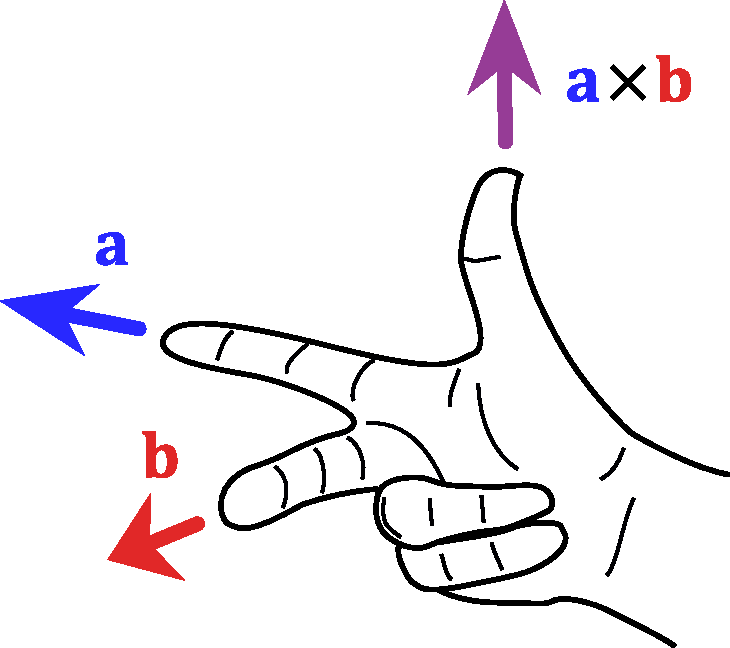
\includegraphics[width=0.3\textwidth]{chapters/vectors/images/right_hand_rule.pdf}
\end{wrapfigure}
\subparagraph{Right-hand rule} The right-hand rule is a simple way to imagine the direction of the vector resulting off a cross product, indeed it is not easy to find it through the Magnitude-Angle notation, nor it is so through Component notation (even though by crunching the numbers it is possible to do so). If done well it is easy to visualize how impossible it is to process the same result by switching the arguments: spoiler it would be of the opposite direction.
    \newpage
    \documentclass{scrartcl}

\usepackage{amsthm}
\usepackage{amsmath}
\usepackage{amssymb}
\usepackage{siunitx}

\begin{document}
    \section{1D Motion}
	The rock rocks
\end{document}
    \newpage
    %... so on for all the other chapters
    \section{Motion in Two and Three dimensions}
\paragraph{Basic definitions}\ 

\begin{tabularx}{\textwidth}{l | X | l}
    Quantity & Equation & Units\\
    \hline\hline
    Position & \tabeq{
        \vec{r} = x\hat{i}+y\hat{j}+z\hat{k}}
        &$\si{\metre}$\\
    \hline
    Displacement & \tabeq{
        \Delta\vec{r}=\begin{cases}
            \vec{r_2} - \vec{r_1}\\
            (x_2 - x_1) \hat{i} + (y_2 - y_1) \hat{j} + (z_2 - z_1) \hat{k}
        \end{cases}}&$\si{\metre}$\\
    \hline
    Velocity & \tabeq{
        \vec{v}_{\mathrm{avg}} =\begin{cases}
            \frac{\Delta\vec{r}}{\Delta t}\\
            \frac{\Delta x}{\Delta t} \hat{i} + \frac{\Delta y}{\Delta t} \hat{j} + \frac{\Delta z}{\Delta t} \hat{k}
        \end{cases}}&$\si{\metre\per\second}$\\
    \hline
    Instantaneous velocity & \tabeq{
        \vec{v} =\begin{cases}
            \frac{d\vec{r}}{dt}\\
            v_x= \frac{dx}{dt},\quad v_y= \frac{dy}{dt},\quad v_z= \frac{dz}{dt}
        \end{cases}}&$\si{\metre\per\second}$\\
    \hline
    Acceleration & \tabeq{
        \vec{a}_{\mathrm{avg}} =\frac{\vec{v}_2 - \vec{v}_1}{\Delta t} = \frac{\Delta \vec{v} }{\Delta t}}&$\si{\metre\per\square\second}$\\
    \hline
    Instantaneous acceleration & \tabeq{
        \vec{a} =\begin{cases}
            \frac{d\vec{v}}{dt}\\
            a_x = \frac{dv_x}{dt},\quad a_y = \frac{dv_y}{dt},\quad a_z = \frac{dv_z}{dt}
        \end{cases}}&$\si{\metre\per\square\second}$\\
    \hline
\end{tabularx}
\paragraph{Applications}
\subparagraph{Projectile motion}\ 

\begin{tabularx}{\textwidth}{l | X}
    Name & Equation \\
    \hline\hline
    Projectile motion & \tabeq{
        \vec{v}_0 = v_{0x} \hat{i} + v_{0y} \hat{j}\ \leftarrow\ v_{0x} = v_0 \cos \theta_0,\quad v_{0y} = v_0\sin\theta_0}\\
    \hline
    Horizontal motion & \tabeq{
        x - x_0 = v_{0x}t}\\
    \hline
    Vertical motion & \tabeq{
        y - y_0 = v_{0y}t - \frac{1}{2}gt^2}\\
    \hline
    Final velocity & \tabeq{
        v_y = v_{0y} - gt\qquad v^2_y = v_{0y}^2 - 2g(y-y_0)}\\
    \hline
    Path's equation & \tabeq{
        y = (\tan \theta_0)x - \frac{gx^2}{2v_{0x}^2}}\\
    \hline
    Horizontal range & \tabeq{
        R = \frac{v^2_0}{g} \sin(2\theta_0)}\\
    \hline
\end{tabularx}
\subparagraph{Uniform circular motion}\ 

\begin{tabularx}{\textwidth}{l | X}
    Name & Equation \\
    \hline\hline
    Centripetal acceleration & \tabeq{
        a_c = \frac{v^2}{r}}\\
    \hline
    Period & \tabeq{
        T = \frac{2\pi r}{v}}\\
    \hline
\end{tabularx}

\subparagraph{Relative motion}\ 

\begin{tabularx}{\textwidth}{l | X}
    Name & Equation \\
    \hline\hline
    Relative position & \tabeq{
        \vec{r}_{\mathrm{PA}} = \vec{r}_{\mathrm{PB}} + \vec{r}_{\mathrm{BA}}}\\
    \hline
    Relative velocity & \tabeq{
        \vec{v}_{\mathrm{PA}} = \vec{v}_{\mathrm{PB}} + \vec{v}_{\mathrm{BA}}}\\
    \hline
    Relative acceleration & \tabeq{
        \vec{a}_{\mathrm{PA}} = \vec{a}_{\mathrm{PB}}}\\
    \hline
\end{tabularx}
    \newpage
    \documentclass{scrartcl} % This is the documentclass DONT-TOUCH-THIS


%   Force and Motion I section - by Dario Loi
%   Document produced through refactoring (shameless theft)
%   of vectors_table.tex

%   remove unnecessary imports from the document when merging!


\usepackage{amsthm}
\usepackage{amsmath}
\usepackage{amssymb}
\usepackage{siunitx}
\usepackage{nicefrac}
\usepackage{tabularx}
\usepackage{graphicx}
\usepackage{wrapfig}

\newcommand{\tabeq}[1]{\parbox[c]{\hsize}{\begin{equation*}#1\end{equation*}}}

\sisetup{
    quotient-mode = fraction,
    per-mode = fraction,
    fraction-function=\nicefrac
}

% Defining the title of the doc.
\title{Physics' formulary}
\subtitle{by and for the Sapienza's ACSAI 2020/21 students}
\date{}

\begin{document}
\section{Force and Motion}

\subsection{Chapter I}
\paragraph{Units of Measurement}\ 

\begin{tabularx}{\textwidth}{l | X | X}
    Quantity & Unit & Formula\\
    \hline\hline
    Force 
    & \tabeq{ 
        [N] = Newton
        } 
    & \tabeq{
        N = Kg * \frac{m}{s^2}
        } \\
        

    \hline

\end{tabularx}
\paragraph{Newton's laws}\ 

\begin{tabularx}{\textwidth}{l | X}
    Law & States \\
    \hline\hline
    First law 
    & \tabeq{ 
        \vec{F}_{net} = 0 \iff v = const
        }  \\
    \hline
    Second law 
    & \tabeq{ 
        \vec{F}_{net} = m\vec{a}
        }  \\
    \hline
    Third law 
    & \tabeq{ 
        \vec{F}_{AB} = -\vec{F}_{BA}
        }  \\
    \hline
    
    
\end{tabularx}
\subsection{Chapter II}
\paragraph{Friction}\ 

\begin{tabularx}{\textwidth}{l | X}
    Type & Formula \\
    \hline\hline
    Static friction
    & \tabeq{ 
        f_{s,max} = \mu_s F_N
        }  \\
    \hline
    Kinetic friction
    & \tabeq{ 
        f_{k} = \mu_k F_N
        }  \\
    \hline
    
\end{tabularx}

\paragraph{Uniform Circular Motion}\ 

\begin{tabularx}{\textwidth}{l | X}
    Quantity & Formula \\
    \hline\hline
    Acceleration
    & \tabeq{ 
        a = \frac{v^2}{R}
        }  \\
    \hline
    Force
    & \tabeq{ 
        F = m\frac{v^2}{R}
        }  \\
    \hline
    
\end{tabularx}

\end{document}
    \newpage
    
\section{Kinetic Energy and Work}
\paragraph{Basic Definitions}\

\begin{tabularx}{\textwidth}{l | X | l}
Quantity & Equation & Units \\
\hline\hline
Kinetic Energy & \tabeq{\frac{1}{2}mv^2}& J \\
 \hline
\makecell[l]{Work Done by a\\Constant Force} &\tabeq{W=\vec{F}\cdot \vec{d}= Fd \cos\phi} & $\si{\newton\times\metre}=\si{\joule}$ \\ 
 \hline
 Average Power & \tabeq{ P_{\mathrm{avg}} = \frac{W}{\Delta t}} & $\si{\watt}$\\
 \hline
 Instantaneous Power & \tabeq{
     P = \frac{dW}{dt}
 } & $\si{\watt}$ \\
 \hline
 Spring Force & \tabeq{
     F_s = -kx
 } & $\si{\newton}$ \\
 \hline
\end{tabularx}


\paragraph{Applications}\

\begin{tabularx}{\textwidth}{l | X }
Name & Equation \\
\hline\hline
\makecell[l]{Work-Kinetic Energy Theorem} &\tabeq{\Delta K = K_f - K_i = W}\\
\hline
\makecell[l]{Work fone by the\\Gravitational Force }& \tabeq{
    W_g =\vec{F}_g\cdot\vec{d}=mgd\cos \phi}\\
\hline
\makecell[l]{Work done in lifting\\and lowering an object}& \tabeq{
    \Delta K = K_f - K_i = W_a + W_g
}\\
\hline
\makecell[l]{Work done by a Spring force}& \tabeq{
    W_s = \frac{1}{2}kx_i^2 - \frac{1}{2}kx_f^2} \\
\hline
\makecell[l]{Work by a general\\variable force}& \tabeq{W =\begin{cases} \int_{x_i}^{x_f} F (x) \, dx\\
    \int_{x_i}^{x_f} F_x \, dx + \int_{y_i}^{y_f} F_y \, dy + \int_{z_i}^{z_f} F_z \, dz \end{cases}}\\
\hline
\makecell[l]{Instantaneous Power\\at an angle $\phi$}& \tabeq{P =\vec{F} \cdot \vec{v}= Fv \cos\phi} \\
\hline
\end{tabularx}
    \newpage
    \section{Rotation}
\paragraph{Basic definitions}\ 

\begin{tabularx}{\textwidth}{l | X | l}
    Quantity & Equation & Units\\
    \hline\hline
    Angular Position & \tabeq{
        \theta=\frac{s}{r}, \mbox{ where }\begin{cases}
            s\mbox{ is portion of circumference}\\
            r\mbox{ is radius}
        \end{cases}}
        &$\si{\radian}$\\
    \hline
    Angular displacement & \tabeq{
        \Delta\theta =\theta_2 - \theta_1}&$\si{\radian}$\\
    \hline
    Angular velocity & \tabeq{
        \omega_{\mathrm{avg}} = \frac{\Delta\theta}{\Delta t}}&$\si{\radian\per\second}$\\
    \hline
    Instantaneous angular velocity & \tabeq{
        \omega = \frac{d\theta}{d t}}&$\si{\radian\per\second}$\\
    \hline
    Angular speed & \tabeq{
        |\omega|}&$\si{\radian\per\second}$\\
    \hline
    Average angular acceleration & \tabeq{
        \alpha_{\mathrm{avg}}=\frac{\Delta\omega}{\Delta t}}&$\si{\radian\per\square\second}$\\
    \hline
    Instantaneous angular acceleration & \tabeq{
        \alpha = \frac{d\omega}{dt}}&$\si{\radian\per\square\second}$\\
    \hline
\end{tabularx}

\subparagraph{Derivations}\ 

\begin{tabularx}{\textwidth}{l | X }
    Name & Equation \\
    \hline\hline
    Angular velocity I & \tabeq{\omega = \omega_0 + \alpha t}\\
    \hline
    Angular position & \tabeq{(\theta-\theta_0) = \omega t + \frac{1}{2}\alpha  t^2}\\
    \hline
    Angular velocity II &\tabeq{\omega^2 = \omega_0^2 + 2\alpha (\theta-\theta_0)}\\
    \hline
    Speed & \tabeq{v=\omega r}\\
    \hline
    Tangential acceleration & \tabeq{a_t = \alpha r}\\
    \hline
\end{tabularx}

\paragraph{Applications}\ 

\begin{tabularx}{\textwidth}{l | X}
    Name & Equation \\
    \hline\hline
    Rotational inertia & \tabeq{I = \sum_i m_i r_i^2}\\
    \hline
    Rot. inertia continuous bodies & \tabeq{I = \int r^2\ dm}\\
    \hline
    Kinetic energy & \tabeq{K = \frac{1}{2} I \omega^2}\\
    \hline
\end{tabularx}
    \newpage
    
\section{Gravitation}
\paragraph{Constants}\

\begin{tabularx}{\textwidth}{l | X}
  Constant & Value\\
  \hline\hline
  Gravitational constant&\tabeq{G = \begin{cases}
    \SI{6.67E-11}{\newton\metre\per\square\kilogram}\\
    \SI{6.67E-11}{\cubic\metre\per\kilogram\per\square\second}
  \end{cases}}\\
  \hline
\end{tabularx}
\paragraph{Equations}\ 

\begin{tabularx}{\textwidth}{l | X}
    Notation & Equation\\
    \hline\hline
    Gravitational force's magnitude & \tabeq{F = G\frac{m_1 m_2}{r^2}}\\\hline
    \makecell[l]{Gravitational force from\\multiple objects (superposition)}& \tabeq{
    \vec{F}_{1,\mathrm{net}} = \vec{F}_{1,2}+ \vec{F}_{1,3} + \dots + \vec{F}_{1,n}  =  \sum_{i=2}^{n} \vec{F}_{1,i}}\\
    \hline
    \makecell[l]{Superposition on an\\extended real object}& \tabeq{
     \vec{F}_{1} = \int \vec{F}(x)\ d\vec{F}}\\
    \hline
    \makecell[l]{Gravitational acceleration\\from a (celestial) body}& \tabeq{a_g =  \frac{GM}{r^2}}\\\hline
    
    \makecell[l]{Newton's second law\\for forces along r-axis}& \tabeq{F_N - ma_g = -m\omega^2 R}\\\hline
    
    \makecell[l]{Free-fall acceleration\\(near Earth's surface)}&\tabeq{g=a_g-\omega^2 R}\\\hline
       
    Gravitational force inside Earth& \tabeq{F = \frac{GMm}{R^3} r}\\\hline
    
    \makecell[l]{Gravitational potential energy\\between two particles}& \tabeq{U =-\frac{Gm_1m_2}{r}}\\\hline
    
    \makecell[l]{Gravitational potential energy\\between multiple particles}& \tabeq{U_{\mathrm{TOT}}= U_{1,2} + U_{1,3} + \dots + U_{1,n} + U_{2,3} + \dots + U_{2,n} + \dots}\\\hline
    
    \makecell[l]{Change of potential\\gravitational energy (path indep.)}& \tabeq{\Delta U = U_f - U_i = -W}\\\hline
    
    Escape velocity&\tabeq{v =\sqrt{\frac{2GM}{R}}}\\
    \hline
\end{tabularx}
    \newpage
    
%Done by Davide di Trocchio, 1940108, 5/12. 
%This table follows (Halliday: 19.1, 19.2, last part of 19.9) as written on the elearning by the professor. 
%It is based on benjamin's tables, just to have a standard to refer to. 
%Further formulas were not included to reduce confusion. If necessary just say so, i'll add them ASAP
%Also some of the equations do not have units, they need some fact-checking. ty <3
%Note that \end{tabularx} throws an error, idk why but it builds just fine so i didn't bother much. 
\section{Kinetic Theory of Gases}
\paragraph{Basic Definitions}\

\begin{tabularx}{\textwidth}{l | X | l}
Quantity & Equation & Units \\
\hline
Avogadro's number & \tabeq{N_{A} = \num{6.02e23}} & $\si{\per\mole}$ \\\hline
Universal Gas constant & \tabeq{R=\num{8.3145}} & $\si{\joule\per\mole\per\kelvin}$ \\\hline
Boltzmann's constant & \tabeq{k_B = \frac{R}{N_A} = \num{1.38e-23}} & $\si{\joule\per\kelvin}$ \\\hline
Mole & \tabeq{M = mN_A}& $\si{\mole}$ \\\hline
Number of moles & \tabeq{n = \frac{N}{N_A} = \frac{M_\mathrm{sam}}{M} = \frac{M_\mathrm{sam}}{mN_A}}& $\si{\mole}$ \\\hline
Ideal Gas Law & \tabeq{pV = nRT} & \\\hline
Ideal Gas Law by Boltzmann's constant & \tabeq{pV = N_A k_BT} & \\\hline
Free Expansion (adiabatic and isothermal) & \tabeq{pV = \mbox{constant}}\\\hline
\end{tabularx}
\paragraph{Applications}\

\begin{tabularx}{\textwidth}{l | X }
Name & Equation\\\hline
Work done by an Ideal Gas &\tabeq{W = nRT\ln{\frac{V_f}{V_i}}}\\\hline
\dots at constant volume & \tabeq{W = 0}\\\hline
\dots at constant pressure & \tabeq{W = p\int_{V_i}^{V_f} \ dV = p\Delta V}\\\hline
\end{tabularx}
    \newpage
    \section{Gauss' Law}
\paragraph{Gauss Law}\


\begin{tabularx}{\textwidth}{l | X}
     Law & Formula\\
     \hline\hline
     Gauss' Law 
     & \tabeq {
        \epsilon_{0}\Phi = q_{enc}
     }\\
     \hline
     Flux through a flat face
     & \tabeq {
        \Delta\Phi = \vec{E}\cdot \Delta A = |E|\cdot\Delta A\cdot\cos\alpha
     }\\
     \hline
     Flux through any Gaussian surface
     & \tabeq {
        \Phi = \oint \vec{E}\cdot d\vec{A}
     }\\\hline
\end{tabularx}
\paragraph{Applications}\

\begin{tabularx}{\textwidth}{l | X}

    Description & Formula\\
    \hline\hline
    Electric field due to a charged surface 
    & \tabeq{
        E = \frac{\sigma}{\epsilon_{0}}
    }\\
    \hline
    Elec. field due to a charged line
    & \tabeq{
        E = \frac{\lambda}{2\pi\epsilon_{0}r}
    }\\
    \hline
    Elec. field due to a charged sheet
    & \tabeq{
    E = \frac{\sigma}{2\epsilon_{0}}
    }\\
    \hline
    \makecell[l]{Elec. field from due to a spherical shell\\(i.e same as Coulomb's)}
    & \tabeq{
    E=\frac{1}{4\pi\epsilon_{0}} \frac{q}{r^2}
    }\\\hline
\end{tabularx}
\end{document}
